\documentclass[../entwurf.tex]{subfiles}

\begin{document}
\section{Starten eines Songs aus der Audiobibliothek}
\begin{center}
	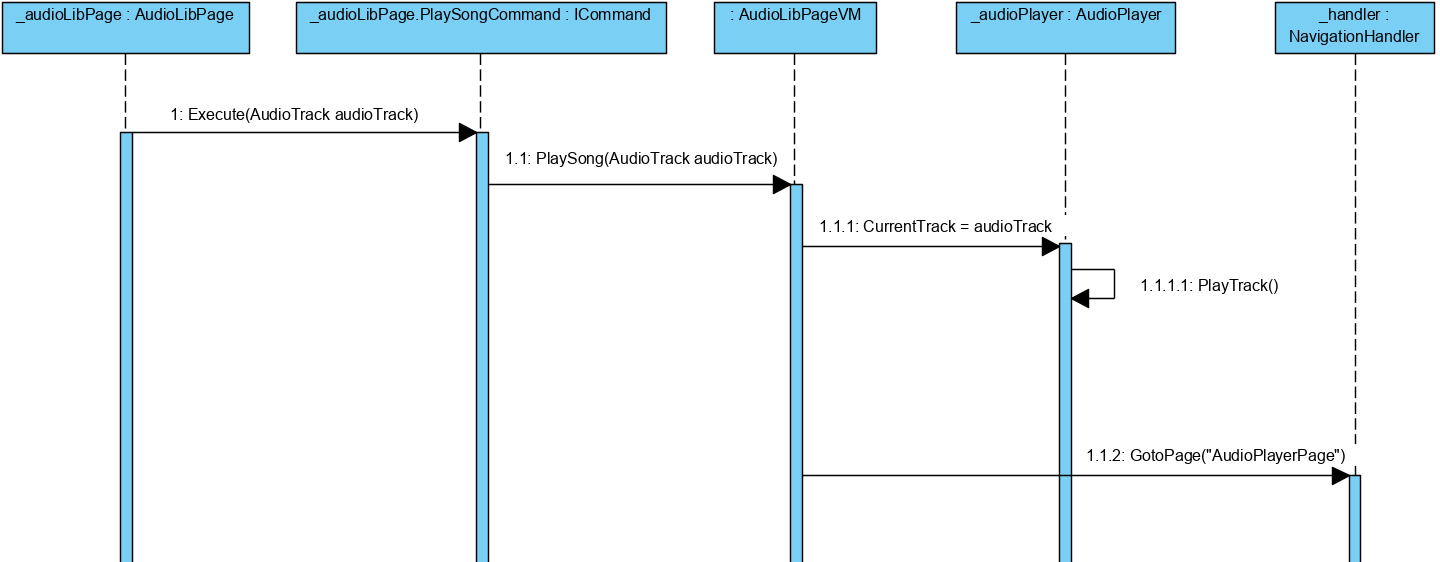
\includegraphics[page=1,width=350pt,keepaspectratio]{../graphics/sequenz_diagramme/PlaySongSequenzDia.png}
\end{center}
Das Sequenz-Diagramm stellt dar was passiert nachdem der User auf einen Song in der AudioLibrary gedrückt hat.
\section{Suchen neuer ESense Earables}
\begin{center}
	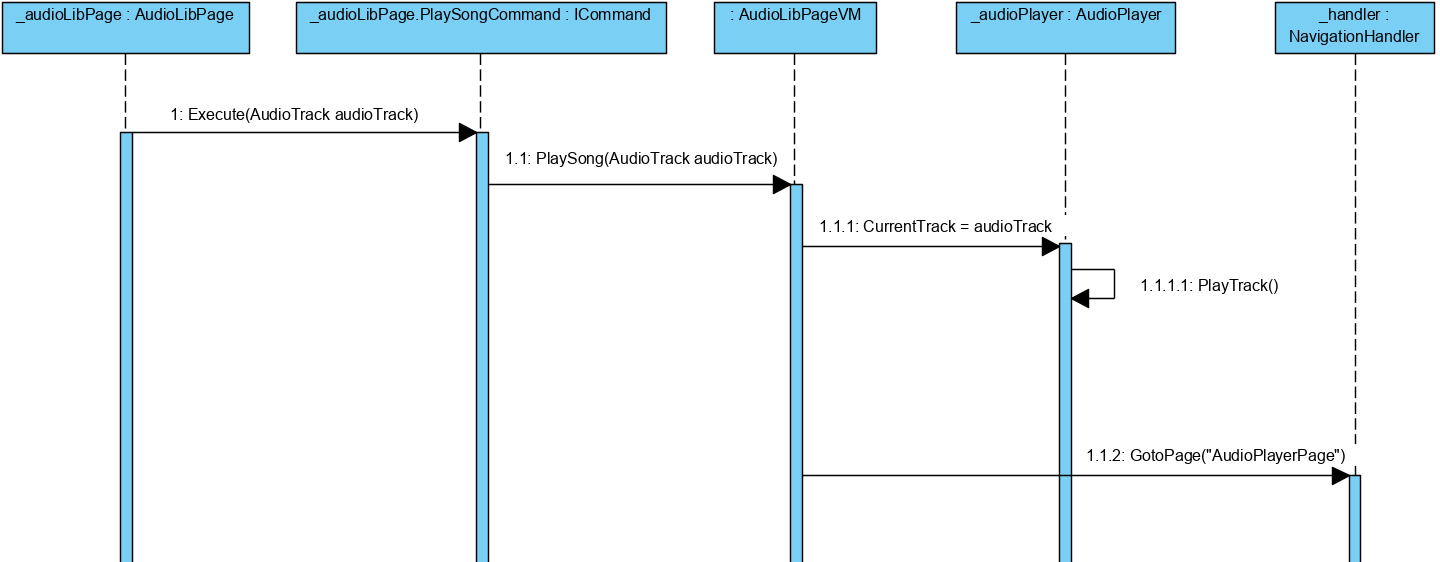
\includegraphics[page=1,width=350pt,keepaspectratio]{../graphics/sequenz_diagramme/PlaySongSequenzDia.png}
\end{center}
Das Sequenz-Diagramm stellt dar was passiert wenn der User auf der ConnectionPage auf den Refresh-Button drückt.
\section{Aktivieren eines Modus}
\begin{center}
	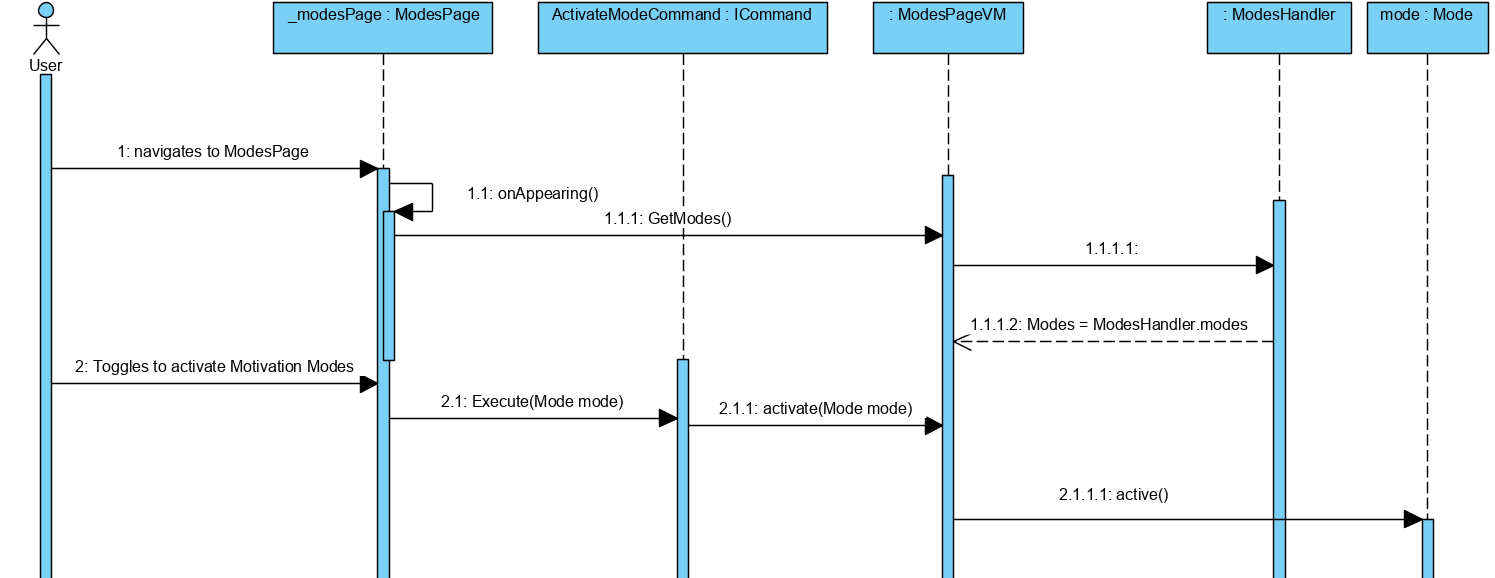
\includegraphics[page=1,width=350pt,keepaspectratio]{../graphics/sequenz_diagramme/ActivateModeDia.png}
\end{center}
Das Diagramm stellt dar was passiert wenn der User auf die ModePage wechselt und einen beliebigen Modus der App aktiviert.
\section{Verwendung des AutoStop Modus}
\begin{center}
	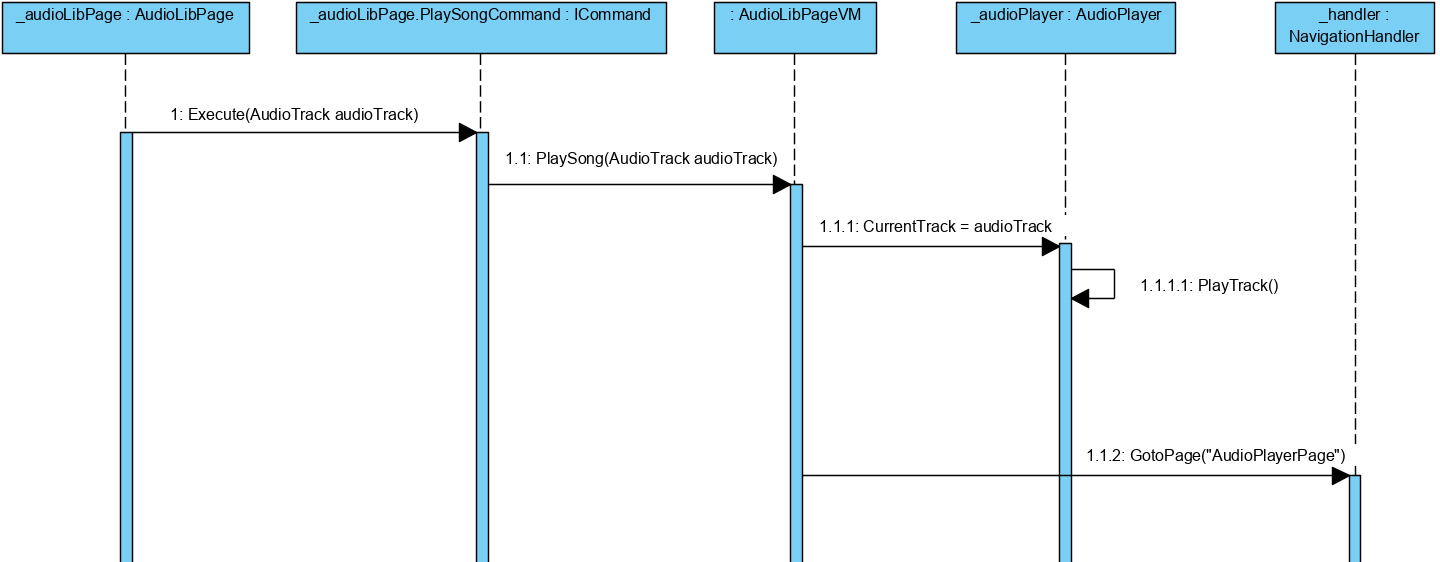
\includegraphics[page=1,width=350pt,keepaspectratio]{../graphics/sequenz_diagramme/PlaySongSequenzDia.png}
\end{center}
Das Sequenz-Diagramm stellt dar was passiert wenn der User den AutoStop-Modus aktiviert hat und stehen bleibt.
\end{document}